%%% template.tex
%%%
%%% This LaTeX source document can be used as the basis for your technical
%%% paper or abstract. Intentionally stripped of annotation, the parameters
%%% and commands should be adjusted for your particular paper - title, 
%%% author, article DOI, etc.
%%% The accompanying ``template.annotated.tex'' provides copious annotation
%%% for the commands and parameters found in the source document. (The code
%%% is identical in ``template.tex'' and ``template.annotated.tex.'')

\documentclass[annual]{acmsiggraph}
\usepackage{program}

\TOGonlineid{45678}
\TOGvolume{0}
\TOGnumber{0}
\TOGarticleDOI{1111111.2222222}
\TOGprojectURL{}
\TOGvideoURL{}
\TOGdataURL{}
\TOGcodeURL{}

\title{Mobile Depth from Focus and Applications}

%\author{Naran Bayanbat\thanks{e-mail:naranb@stanford.edu}\\Stanford University \and Jason Chen\thanks{e-mail:jasonch@stanford.edu} \\Stanford University \and Chun-Wei Lee\thanks{e-mail:chunweil@stanford.edu} \\Stanford University}
\author{Naran Bayanbat\\naranb@stanford.edu\\Stanford University \and Jason Chen\\jasonch@stanford.edu\\Stanford University \and Chun-Wei Lee\\chunweil@stanford.edu\\Stanford University}
\pdfauthor{Naran Bayanbat, Jason Chen, Chun-Wei Lee}

\keywords{depth from focus, depth map, tablet, computational photography}

\begin{document}

 \teaser{
   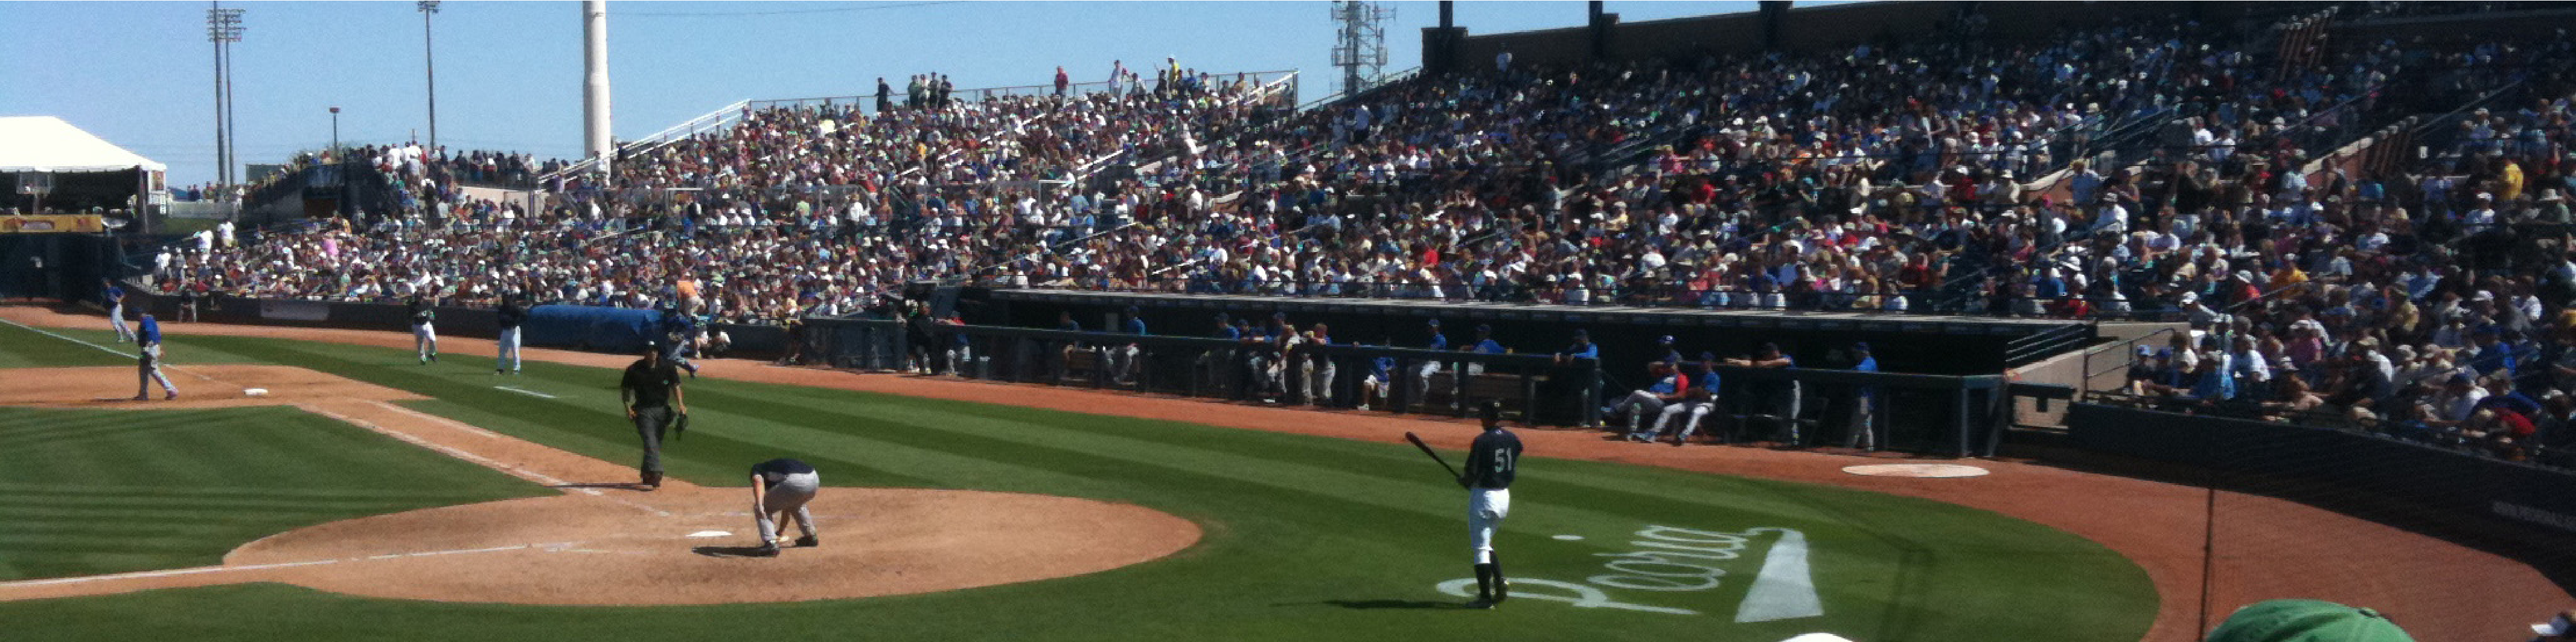
\includegraphics[height=1.5in]{images/sampleteaser}
   %\caption{}
 }

\maketitle

\begin{abstract}
Depth information is crucial in providing scene understanding for many post-processing applications in computational photography. While depth maps can be easily obtained through stereo cameras or external devices such as infrared sensors, it is difficult in mobile photography because of hardware limitation. In this project, we will implement depth-by-focus, sweeping a single lens across various focus distances and composite an approximate depth map. The depth map will be improved by segmentation and bilateral filtering. We will then demonstrate the effectiveness of the technique by utilizaing the depth map and simulate light-field photography as well as synthetic depth of field.

\end{abstract}

\begin{CRcatlist}
  %\CRcat{I.3.3}{Computer Graphics}{Three-Dimensional Graphics and Realism}{Display Algorithms}
  %\CRcat{I.3.7}{Computer Graphics}{Three-Dimensional Graphics and Realism}{Radiosity};
\end{CRcatlist}

\keywordlist

%\TOGlinkslist

\copyrightspace

\section{Introduction}

Mobile devices have become the most common photography means, and they have presented a new set of opportunities and challenges for computational photography.  While many applications take advantage of these devices' location, accelerameter, and other meta data, the inherent hardware limitation on size computation power makes it worth revisiting prior works on computational photography to this application.  Specifically, since depth information is one of the most useful piece of scene understanding, we wish to demonstrate a mobile solution producing a depth map that assist in computational photography.  Since most mobile devices have only one camera (lens) and no active focusing equipment, we will attempt to implement depth from focus, approximating depth information from images captured at different depths. 

\section{Prior Work}

Depth from Focus is a technique that has been studied for decades \cite{Grossmann1987} \cite{pyramid} and with numerous applications, as it is relatively easy to compute and implement and requires no additional hardware.  It is also flexible and can be adjusted for real-time, low resolution depth map \cite{mobileRobot} as well as more detailed depth maps.

\section{Results}

\subsection{Depth Sampling}
At each focus distance, we densely sampled 36x27 square patches of width 30 pixels and calculate the sharpness of each patch.  We tried many different sharpness measures, starting with a simple high pass filter to the Sobel edge detection filter.  After evaluating the results, we concluded Sobel edge detection filter produces the best results. Sobel filter is composed of the horizontal box filter, $G_x$, and the vertical box filter, $G_y$, which are 
\[
G_x = \begin{bmatrix} -1 & 0 & 1 \\ -2 & 0 & 2 \\ -1 & 0 & 1 \end{bmatrix}
G_y = \begin{bmatrix} -1 & -2 & -1 \\ 0 & 0 & 0 \\ 1 & 2 & 1 \end{bmatrix}
\]. For each pixel in the image at $(i,j)$, we compute its sharpness value $l_{x,y}$ as 
\begin{eqnarray}
gx &:=& G_x * I_d[i,j] \nonumber \\
gy &:=& G_y * I_d[j,i] \nonumber \\
l_{i,j} &:=& gx^2 + gy^2 
\end{eqnarray}, where $gx$ is the resulting value after applying the Sobel horizontal box filter, and $gy$ the vertical box filter. Finally, the sharpness $\lambda_{x,y}$ to be the sum of all pixel sharpness $l$ within the patch. \\
As we sweep across different focus distances, we record only the current maximum sharpness and the focus distance at which this is obtained for each sample point. We make the assumption that an object exists at the distance which produces the maximum sharpness response.  Prior works have attempted to interpolate the response curve and estimate the true maximum \cite{Grossmann1987}, but we decided this is unnecessary for our applications and too much computation on a mobile device. 

\subsection{Depth Map Generation}
\label{sec:depthmap-generation}
One of the inherent problem in sharpness calculations, as well as in all focusing methods in general, is that they fail on textureless surfaces.  Therefore, after obtaining the best focus distance and best sharpness pair, $<d_i, \lambda_i>$, for each sample point, we first correct for points sampled at low texture patches.  Every sample point whose sharpness is below some predefined threshold, $\Lambda$, will update its sharpness by finding the most common depth value in the patches around it.  This is achieved by a simple voting scheme: each of the nine pixels will cast a vote for the depth value it represents, and its vote is weighted by its confidence, which is the normalized sharpness value. \\
Then, we simply naively assume the entire patch exists at the same depth, thus generating a blocky depth map as in ~\ref{fig:initial-depth-map} of the same dimension as the input image. Next, we take a full-colored frame from the input stack as reference image, and use joint bilateral filtering to smooth out the patch boundaries.  This is because we want fairly aggressive smoothing while preserving edges from the color space. \\
This gives us our first approximate depth map, as shown in ~\ref{fig:filtered-depth-map}.  We quickly realized that any frame we could choose from the stack could not serve as a good edge reference, because at least some part of the image is out of focus.  We can solve the problem if we had an all-in-focus image, but we could only get a good all-in-focus image if we had a better depth map.  To solve this problem, we iteratively refined our depth map by generating all-in-focus image based on the current depth map ~\ref{fig:depth-map-refining}.  This provides us highly accurate depth map with clear object edges.

\subsection{All-in-Focus Imaging}

One application of having an image stack and an approximate depth map is to produce all-in-focus images.  As mentioned in section ~\ref{sec:depthmap-generation}, an all-in-focus image can also be used to further improve our depth map.  The algorithm to generate all-in-focus images is simple and intuitive.  For each pixel on the final image, we simply sample from the image in the stack as indicated by the closest depth value. I.e., for each pixel $p_{i,j}$, 
\begin{equation} 
p_{i,j} := images[ depthmap_{i,j} ](i,j)
\end{equation}, where images is image stack represented as an array, and depthmap returns values which are indices into the array.  
\subsubsection{Calibration}
There is a subtle problem to solve when merging images at different focus distances: each focus distance has a slight optical magnification.  Images taken at closer focus distances will be magnified by an amount that is dependent on each lens' manufacturing specification.  Fortunately, since this geometric distortion is consistent across all images taken by the same camera, we can calibrate once just once and store the transformation matrices statically. We use calibration images ~\ref{fig:calibration} and hand-label control points that are corresponding in each pair of images. Since this is a non-reflective similarity transform, only two pairs of control points are necessary for each pair of images.  We compute the transformation matrices using the image with the smallest focus distance as base image.  This is because any coordinate in this image will have a correspondence in farther-focused images, but not vice versa.  Each transformation matrix, $C_d\in R^{3x3}$, transforms homogenized target image coordinates $(x,y,1)$ to the coordinates in the image captured at depth $d$, $(x_d,y_d,1)$. So now we revise the equation to be
\begin{eqnarray} 
v &:=& [x,y,1] \nonumber \\
d &:=& depthmap_{i,j}  \nonumber \\
p_{i,j} &:=& images[ d ]( (C_d v)_x, (C_d v)_y)
\end{eqnarray}

\subsection{Synthetic Depth of Field Application}

\subsection{Image Merge and Insertion}

\section{Concolusions and Further Works}

\subsection{Lighting and Shadows}
One prominent problem with our approach is when the image has strong shadows or specular highlights.  These features produce strong edges in the color space, and thus bilateral filtering may assert a different depth value to these section, even though they should be the same.  This is a difficult problem to solve and is present with other attempts of depth from focus \cite[Grossmann1987] and other unaided image segmentation algorithms.  The best solution to alleviate this problem, if we had more time to implement, is to provide an interface for user feedback and lower the confidence of these segments entirely. 


\section*{Acknowledgements}


\bibliographystyle{acmsiggraph}
\bibliography{template}
\end{document}
